\documentclass{beamer}
\usetheme{Frankfurt}
\usepackage{hyperref}
\title{%
  Neural Networks in Autonomous Vehicles \\
  \small Based on "Driving Darwin" program}
\author{Stanisław Deja}
\date{\today}

\begin{document}

\begin{frame}
  \titlepage
\end{frame}

\begin{frame}{Outline}
  \tableofcontents
\end{frame}

\section{Neural Network}
\begin{frame}{What is a Neural Network?}
    \begin{block}{Definition}
    A neural network is an artificial brain. And can be treated as a function 
    \begin{math}
    f_{NN}(IN)=OUT
    \end{math}
  \end{block}

  \begin{figure}
    
\includegraphics[width=0.6\linewidth]{brain.png}
    \caption{Artificial brain = Neural Network}
  \end{figure}
  \begin{itemize}
      \item Get Some Data
      \item \textbf{Input} it to the artificial brain
      \item Read the \textbf{output}
  \end{itemize}
\end{frame}
\section{Cars Brain}
\begin{frame}{What if we give a Neural Network to a car?}
    \begin{alertblock}{First we need to consider following things}

\begin{itemize}
        \item \textbf{Input to the Artificial Brain:} What information should be fed into the system to facilitate learning and decision-making?
        \item \textbf{Handling the Outcome:} Once the artificial brain processes the input, how should the outcomes be utilized or acted upon?
\end{itemize}
\end{alertblock}

\end{frame}
\begin{frame}{Input for the cars brain}
    \begin{columns}
        \column{.6\textheight}
        \begin{block}{Idea}
            \begin{itemize}
                \item Cars navigate roads smoothly without hitting edges.
                \item Focus on car-to-road-edge distance.
                \item Check distance in various directions.
                \item Input them as an array to our Neural Network.
            \end{itemize} 
        \end{block}
        \column{.4\textheight}
         \begin{figure}
            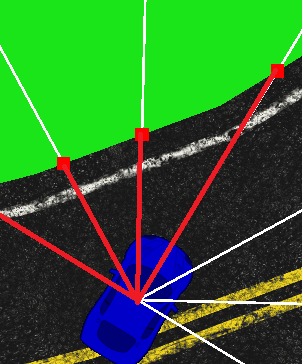
\includegraphics[width=1.0\linewidth]{cardist.png}
            \caption{\tiny Distance to the edge of the road in directions(Red lines)}
        \end{figure}
    \end{columns}
\end{frame}
\begin{frame}{Output of the Network}
    \begin{columns}
        \column{.6\textheight}
        \begin{itemize}
            \item As the brain of our car "knows" about its surroundings
            \item Maybe its good idea to let it steer the car
            \item Let the output of the network be the direction of movement and velocity 
        \end{itemize} 
        \column{.4\textheight}
        \begin{example}
            \begin{figure}
                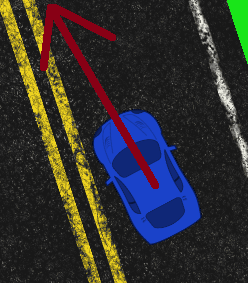
\includegraphics[width=1.0\linewidth]{cardir.png}
                \caption{\tiny Cars brain choses direction and velocity}
            \end{figure}
        \end{example}
         
    \end{columns}
\end{frame}
\begin{frame}{Let's finally give it a brain}
    \begin{columns}
        \column{.6\textheight}
        \begin{block}{Testing the idea}
            \begin{itemize}
                \item Let's finally give it a brain a plug everything in
                \item Put it on the road and...
                \item It bumps into to the edge of the road. \textbf{Why?}
                \item Its brain is very primitive.\textcolor{red}{It needs to learn and evolve} 
            \end{itemize} 
        \end{block}
      
        \column{.4\textheight}
         \begin{figure}
            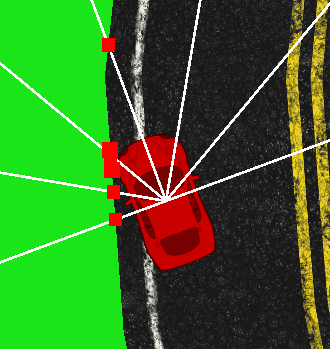
\includegraphics[width=1.0\linewidth]{cardump.png}
            \caption{\tiny Our Car is not very clever for now}
        \end{figure}
    \end{columns}
\end{frame}
\section{Genetic approach}


\begin{frame}{How to make it smarter?}
    \begin{exampleblock}{Simple Idea}
        \centering
        \small{Let’s take a bunch of cars and give each one an unique random brain.}
        \hfill
        \begin{tabular}{c|c|c|c|c|c|c|c}
            
\includegraphics[scale=0.66]{brain0.png}&
            
\includegraphics[scale=0.66]{brain0.png}&
            
\includegraphics[scale=0.66]{brain0.png}&
            
\includegraphics[scale=0.66]{brain0.png}&
            
\includegraphics[scale=0.66]{brain0.png}&
            
\includegraphics[scale=0.66]{brain0.png}&
            
\includegraphics[scale=0.66]{brain0.png}&
            
\includegraphics[scale=0.66]{brain0.png}\\ \hline
            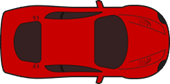
\includegraphics[scale=0.30]{car.png}&
            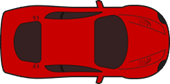
\includegraphics[scale=0.30]{car.png}&
            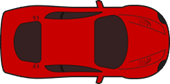
\includegraphics[scale=0.30]{car.png}&
            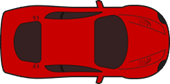
\includegraphics[scale=0.30]{car.png}&
            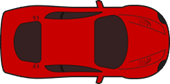
\includegraphics[scale=0.30]{car.png}&
            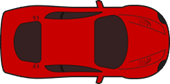
\includegraphics[scale=0.30]{car.png}&
            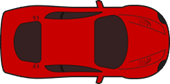
\includegraphics[scale=0.30]{car.png}&
            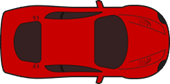
\includegraphics[scale=0.30]{car.png}

        \end{tabular}
        Maybe at least one of them will show some inteligence
    \end{exampleblock}
    \begin{block}{Testing the idea}
        \begin{columns}
        \column{.24\textheight}
        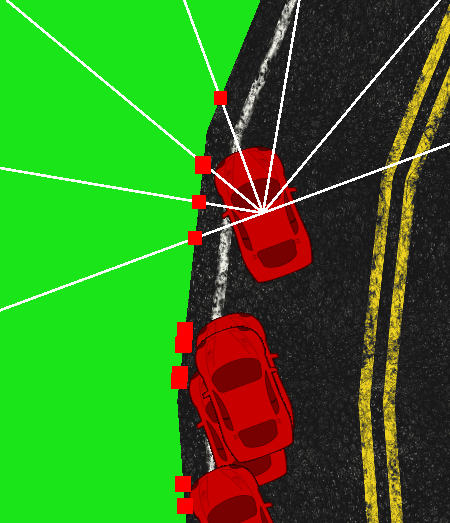
\includegraphics[width=1.3\linewidth]{evolution.png}
        \column{.76\textheight}
        \footnotesize
            \begin{itemize}
                \item Well they still bump into the edge of the road
                \item \textbf{However} One of them managed to travel Further than others
                \item That means its brain was the \textbf{smartest}
                \item Let’s see what we can do with the best car
            \end{itemize}
   
    \end{columns}
    \end{block}

\end{frame}
\begin{frame}{Evolution}
    \begin{block}{New Generation}
        \small{Let’s create a new generation of cars.}
        \hfill
        \begin{tabular}{c|c|c|c|c|c|c|c}
            
\includegraphics[scale=0.66]{brain0.png}&
            
\includegraphics[scale=0.66]{brain0.png}&
            
\includegraphics[scale=0.66]{brain0.png}&
            
\includegraphics[scale=0.66]{brain0.png}&
            
\includegraphics[scale=0.66]{brain0.png}&
            
\includegraphics[scale=0.66]{brain0.png}&
            
\includegraphics[scale=0.66]{brain0.png}&
            
\includegraphics[scale=0.66]{brain0.png}\\ \hline
            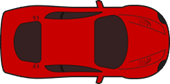
\includegraphics[scale=0.25]{car.png}&
            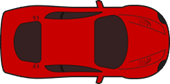
\includegraphics[scale=0.25]{car.png}&
            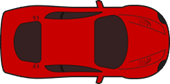
\includegraphics[scale=0.25]{car.png}&
            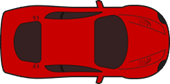
\includegraphics[scale=0.25]{car.png}&
            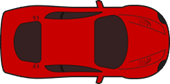
\includegraphics[scale=0.25]{car.png}&
            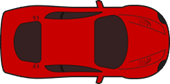
\includegraphics[scale=0.25]{car.png}&
            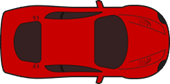
\includegraphics[scale=0.25]{car.png}&
            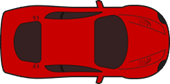
\includegraphics[scale=0.25]{car.png}

        \end{tabular}
        \begin{enumerate}
            \item \textbf{However} this time we will give each new car slightly modified version of
            the best brain from the previous generation.
            \item In that way the new generation will ”learn” from the previous one
        \end{enumerate}
    \end{block}
    \begin{alertblock}{Testing the idea}
        \footnotesize
            \begin{itemize}
                \item We can repeat process described above over and over again
                \item That way each new generation will learn from its predecessors
                \item and stack its knowledge, until...
                \item eventually, we will get a car that is able to drive on its own
            \end{itemize}
    \end{alertblock}
  

\end{frame}

\begin{frame}{Progress over Generation}
    \begin{columns}
        \column{.6\textheight}
        \begin{exampleblock}{Each generation makes progress}
            \centering
         \begin{figure}
            
            \begin{tabular}{c | c}
                Generation & Distance \\
                \hline
                1  & 12\\
                \hline
                2  & 34\\
                \hline
                3  & 52\\
                \hline
                4  & 54\\
                \hline
                5 & 61\\
                \hline
                6 & 91\\
                \hline
                7 & inf\\
            \end{tabular}
        \caption{\tiny{Data collected on 21.12.2023 using ”DrivingDarwin” program}}
        \end{figure}
        \end{exampleblock}
        \column{.4\textheight}
        \begin{itemize}
            \item \footnotesize{Each generation gets better score than the previous}
            \item \footnotesize{Until generation 7 is able to fully drive on the road}
        \end{itemize}
        
  
        
    \end{columns}
\end{frame}

\section{End}
\begin{frame}{Further Reading}
    \begin{block}{Project links}
        \begin{tabular}{c|c}
           \textbf{\footnotesize{Project page* }}&\footnotesize{ \url{https://github.com/stachurski2k/DrivingDarwin}}
        \end{tabular}
    \end{block}
    \begin{block}{Sources}
        \begin{tabular}{c|c}
\textbf{\scriptsize{Inspiration}} & \scriptsize{ \url{https://youtu.be/hfMk-kjRv4c?si=KWKiRY9hVDP_R-bV}}\\
\hline
\textbf{\scriptsize{Neural Networks}} & \scriptsize{ \url{https://youtu.be/aircAruvnKk?si=-pxO5wa7qVt-1eHh}}\\
\hline
\textbf{\scriptsize{Road Generation}}& \scriptsize{ \url{https://youtu.be/RF04Fi9OCPc?si=GgaL0ujYB1aqEibW}}\\
        \end{tabular}
    \end{block}
    \footnotesize{
    * ”Driving Darwin” was fully developed by the author of this presentation, it covers
    much more advanced concepts than presented such as implementation of Neural
    Network from scratch and generator of bezier curves. Their description can be found
    in the documentation of the project.}
\end{frame}

\begin{frame}{Thank You for Your Attention}
    \centering
    \textbf{\underline{\Huge{Any Questions?}}}\\
    by Stanisław Deja
\end{frame}


\end{document}
